In the following, we describe the detailed implementation of the proposed architecture in Chapter~\ref{sec:architecture}.

\subsection{System wide fine design}\label{subsec:system-wide-design}

\subsubsection{Data Transfer Objects (DTOs)}
The \textit{DTO}s are classes that correspond to the request-bodies and response-bodies as declared in the REST-api. \newline
Due to the fact that these classes will be used in all components, i.e.\ server and client, it makes sense to define these as general as possible.
We used only primitive data types and only properties to ensure compatability across all programming languages. \newline
The simplicity of the DTOs allowsus to use automatic serialization from- and into JSON format.
The \textit{DTO}s are visualized in Figure~\ref{fig:dtos}.

\begin{figure}
    \centering
    \fbox{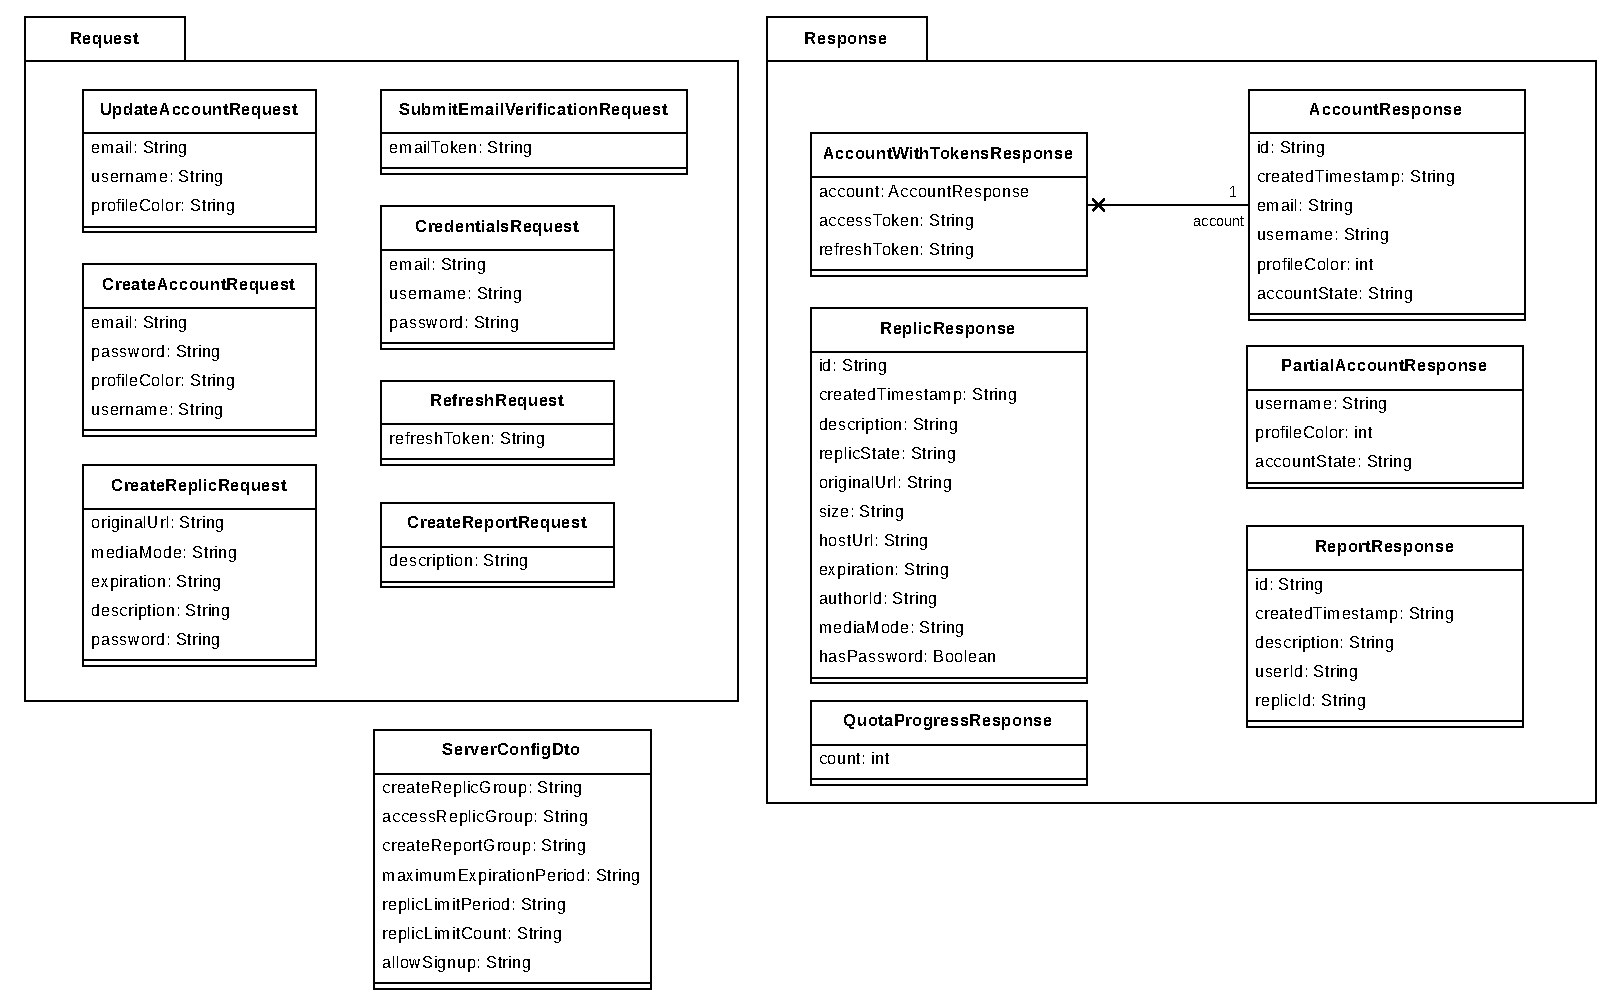
\includegraphics[angle=90,width=\linewidth]{dtos}}

    \caption{Data Transfer Objects}
    \label{fig:dtos}
\end{figure}

\subsubsection{Authentication flow}
Clients will be authenticating themselves with \textit{Json-Web-Tokens} (JWTs) \footnote{https://www.jwt.io/}.

\paragraph{JWTs}
A \textit{JWT} is a string with the following structure: \newline
\begin{center}
    \textit{\textless base64(header)\textgreater.\textless base64(payload)\textgreater.\textless signature\textgreater}
\end{center}

\subparagraph{Header}
The header is a json-object containing the attributes \texttt{alg} ("Algorithm") and \texttt{typ} ("Type of token").
In our case, this header will look like:
\begin{verbatim}
    {
        "alg": "HS256",
        "typ": "jwt"
    }
\end{verbatim}

\subparagraph{Payload}
The payload is a json-object that can contain a selection of attributes.
In our case, the payload will contain the following attributes:
\begin{itemize}
    \item \texttt{iss}: Constant value of \("\)replic-read-server\("\)
    \item \texttt{exp}: ISO-8601 timestamp of the expiration time of the JWT\@.
    \item \texttt{sub}: The id of the account the JWT is created for.
\end{itemize}

\subparagraph{Signature}
The signature is created from the header and payload in the following way: \newline
\begin{center}
    \begin{verbatim}
        HMACSHA256(
        base64(header) + "." +
        base64(payload),
        kessecretret
        )
    \end{verbatim}
\end{center}
where \texttt{secret} is a private key, longer than 256 bits. \newline
Signing the JWT with a private key guarantees the server, that, when presented a JWT by a client, the payload has not been changed.

\paragraph{Logging in}
When a client wants to authenticate, a request with the credentials is sent to \texttt{/auth/login/}.
The server saves a new \textit{refresh-token} and creates a new \textit{JWT} for the client, and returns both these tokens. \newline
Figure~\ref{fig:logging-in} visualizes this flow.

\begin{figure}
    \centering
    \fbox{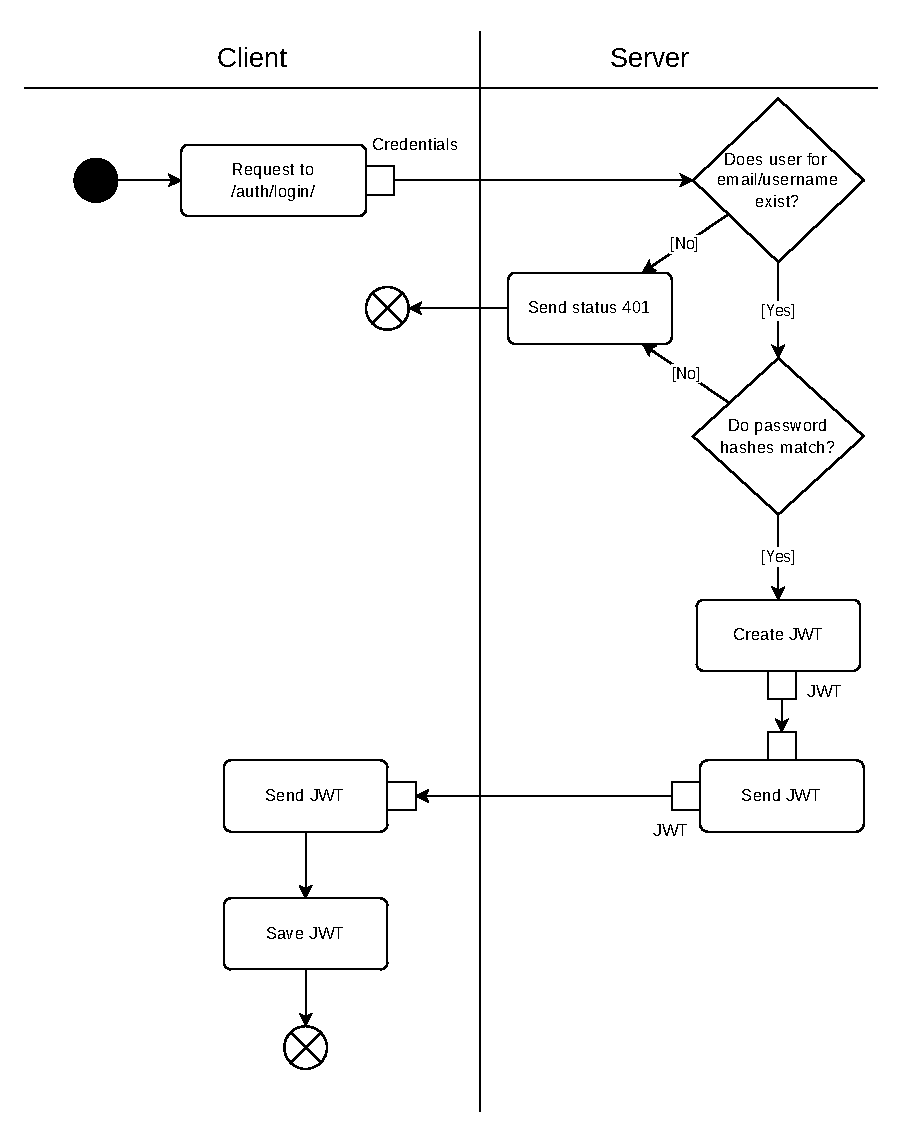
\includegraphics[width=\linewidth]{logging-in}}

    \caption{Flow for logging in}
    \label{fig:logging-in}
\end{figure}

\paragraph{Using an access-token}
When a client wants to perform a request to an endpoint that requires authentication, the \textit{JWT} is included as the value of the \textit{Bearer} header.
Before the requested action is performed, the server checks whether the JWT is valid and non-expired.
If all checks succeed, the action is performed.
If one of the checks fail, status code \textit{401} or \textit{403} is returned. \newline
Figure~\ref{fig:using-access-token} visualizes this flow.

\begin{figure}
    \centering
    \fbox{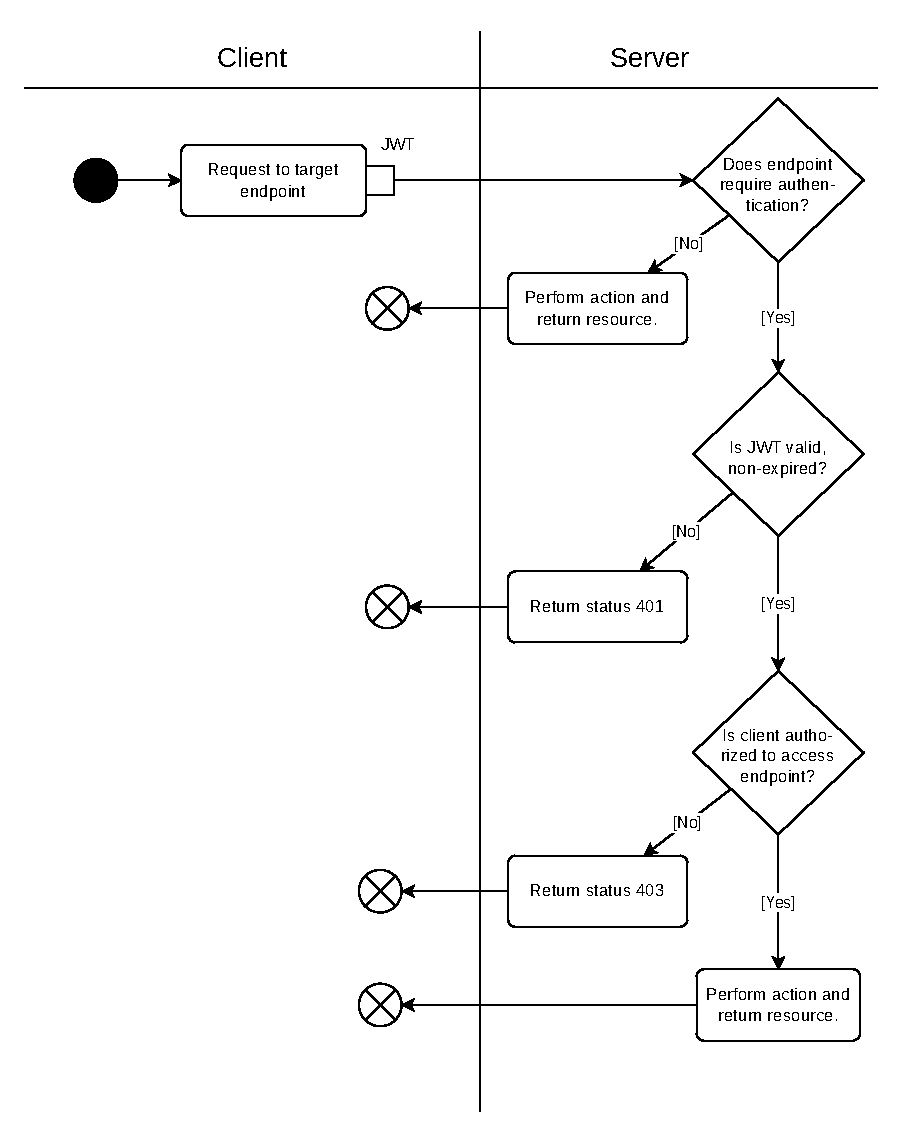
\includegraphics[width=\linewidth]{using-access-token}}

    \caption{Flow for accesing a restricted endpoint}
    \label{fig:using-access-token}
\end{figure}

\paragraph{Using a refresh-token}
When a client wants to create a new access-token using an existing refresh-token, it makes a request to \texttt{/auth/refresh/}.
The server receives the refresh-token and checks whether it exists, is non-expired and non-invalidated.
If all checks succeed, a new refresh-token is created and the old one invalidated.
Together with the new refresh-token, a new access-token is generated and returned.
If one of the checks fail, status \textit{401} is sent. \newline
Figure~\ref{fig:using-refresh-token} visualizes this flow.

\begin{figure}
    \centering
    \fbox{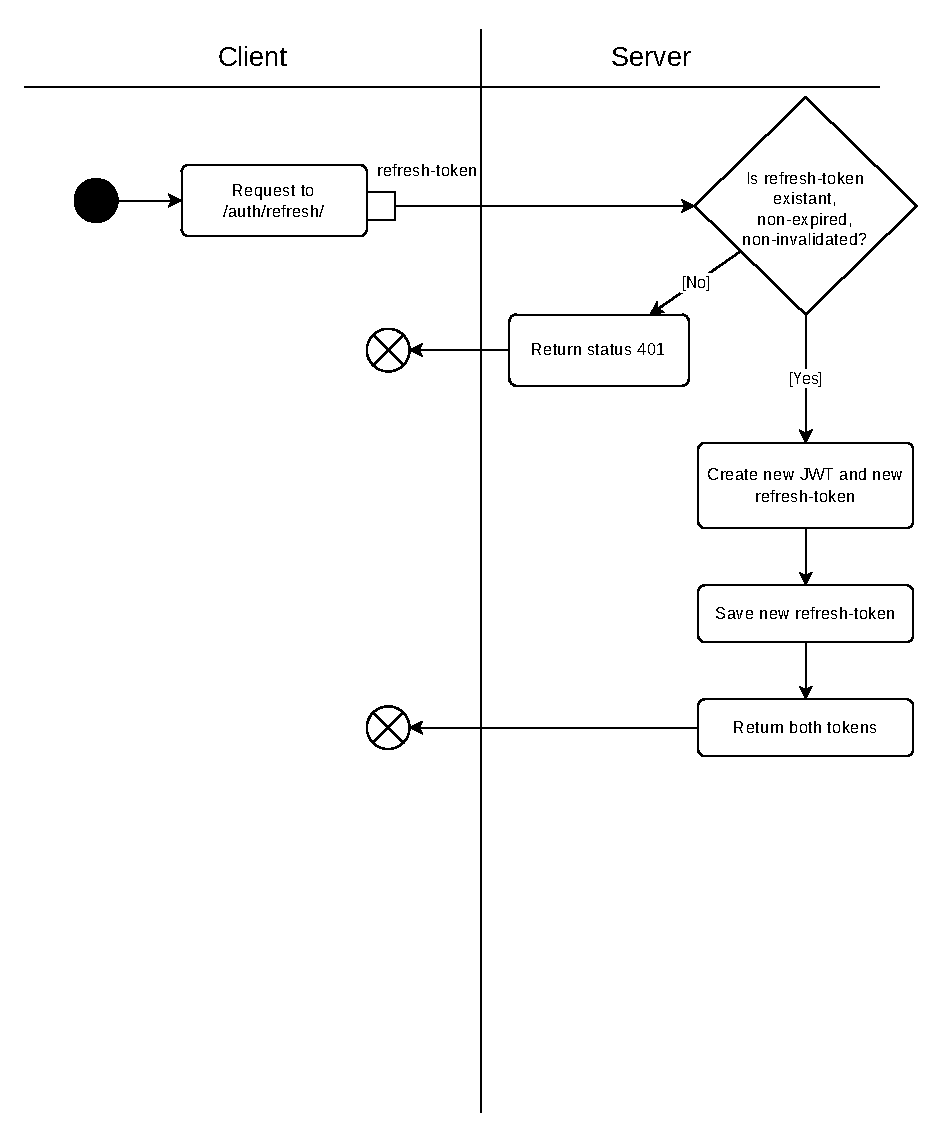
\includegraphics[width=\linewidth]{using-refresh-token}}

    \caption{Flow for refreshing}
    \label{fig:using-refresh-token}
\end{figure}

\subsection{Server fine design}\label{subsec:server-fine-design}

\subsubsection{Configuration}
Aside from the server-config that can be set up inside the admin-panel in the web-client, there are configurations that are not domain-related and will not be available on that panel.
The following options can be configured:
\begin{itemize}
    \item \textit{Server domain:} The url without path where the server is running.
    This is required due to the fact that creating the links to the new replic-content requires knowledge of the full URL to the endpoint of \texttt{/replic/\{id\}/content/}.
    \item \textit{REST-API path:} The root path where the REST-API will be available.
    \item \textit{Access-Token lifespan length:} The length that an access-token is valid.
    \item \textit{Access-Token secret:} The signing secret used to sign the access-tokens.
    \item \textit{Refresh-Token lifespan length:} The length that a refresh-token is valid.
    \item \textit{Database url:} The url where the database is located.
    \item \textit{Database username} The username to connect to the database.
    \item \textit{Database password} The password to connect to the database.
    \item \textit{Mail from:} The sender of the email.
    \item \textit{Mail username:} The username for email authentication.
    \item \textit{Mail password:} The password for email authentication.
    \item \textit{Mail smtp host:} The smtp host for email authentication.
    \item \textit{Mail smtp port:} The smtp port for email authentication.
    \item \textit{Mail SSL:} Whether to use SSL for email authentication.
\end{itemize}
These parameters are provided to the server program externally.

\subsubsection{Internal server interfaces}
In the following, we will present the fine design of the internal server interfaces, as described in~\ref{subsec:internal-server-interfaces}.

\paragraph{Request-Execution}
The \textbf{Request-Execution} interface provides one method for each endpoint and http-method in the \textit{REST-API}.
The method parameters are either request bodies, query parameters or path variables.
The method return values are the response bodies.\newline
The responsibility of the request executors is to ensure authorization by using the authorizer, handling errors that might occur in the services, and converting the results of the services to the response bodies.
Figure~\ref{fig:inter-executors} gives an overview over the interface.
Multiple request executors are provided to isolate independant themes.

\begin{figure}
    \centering
    \fbox{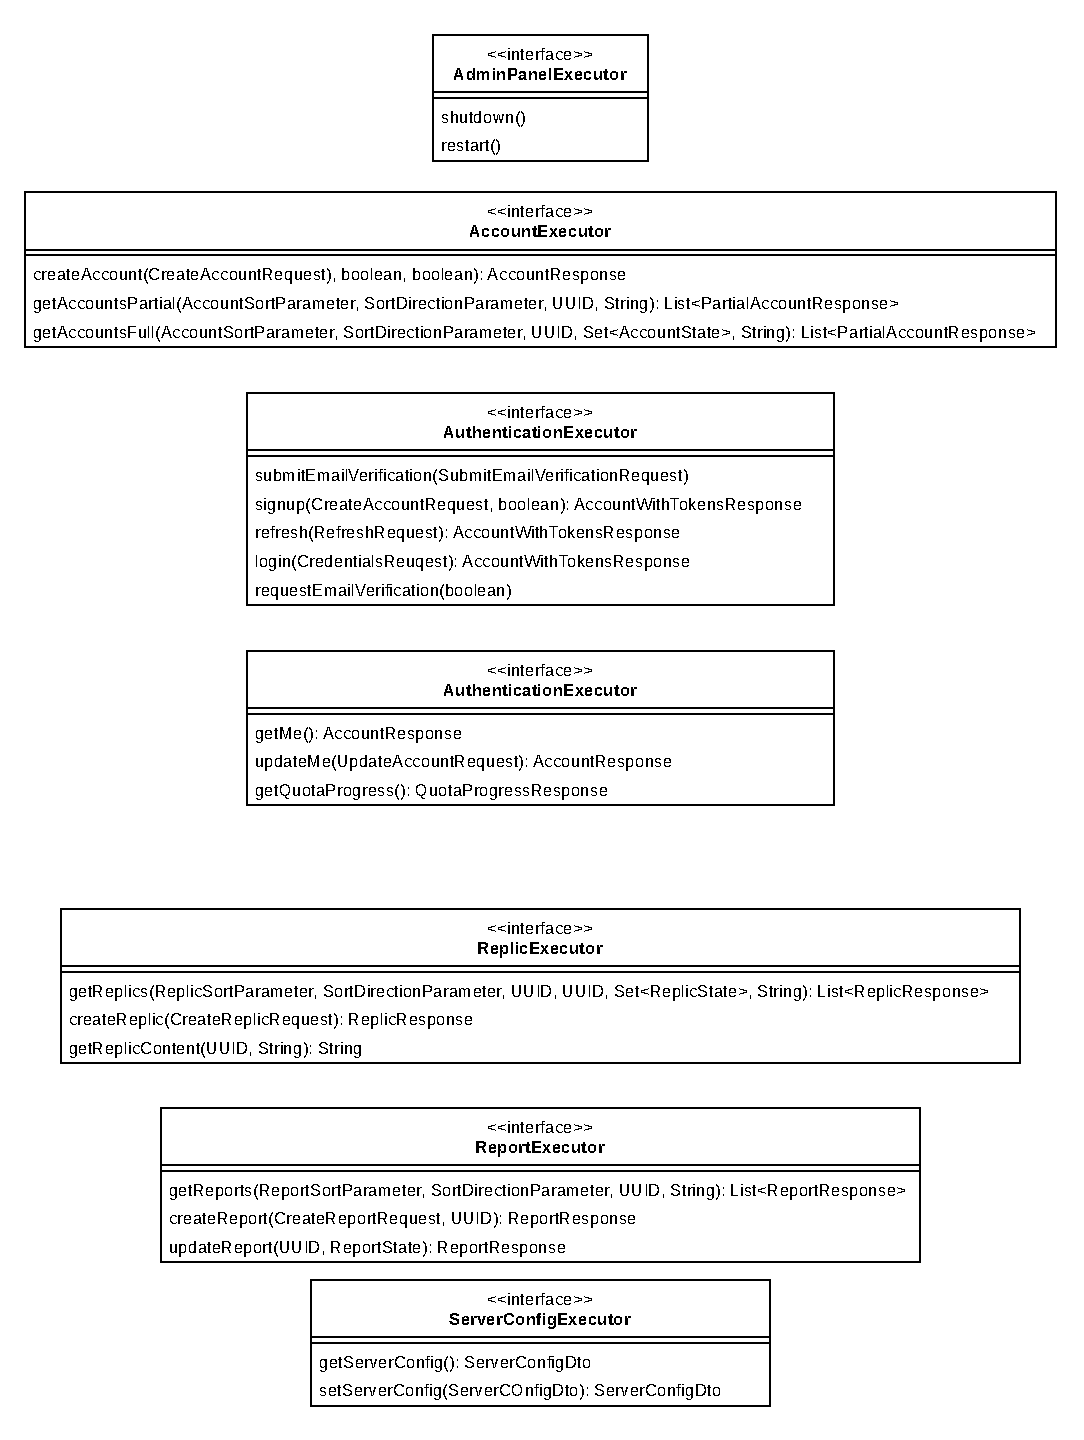
\includegraphics[width=\linewidth]{inter-executors}}

    \caption{Interface for \textit{Request-Execution}}
    \label{fig:inter-executors}
\end{figure}

\paragraph{Authorization}
The \textbf{Authorization} makes the decisions for whether a client, authenticated or anonymous, is allowed to perform a specific request. \newline
In most cases, this comes down to checking whether a client fulfills the auth group set by the config, or whether the client itself is an admin.
Figure~\ref{fig:inter-authorizer} shows the methods of the authorizer interface.

\begin{figure}
    \centering
    \fbox{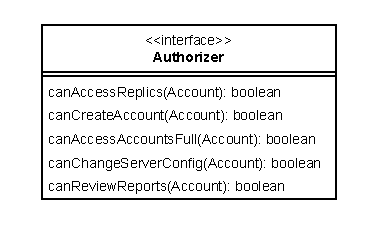
\includegraphics{inter-authorizer}}

    \caption{Interface for \textit{Authorization}}
    \label{fig:inter-authorizer}
\end{figure}

\paragraph{Domain-Models}
The domain models are the basic data classes that model the business structure. \newline
To differentiate between a replic that has been linked to a file vs.\ one that hasn't been, \texttt{Replic} is a specific case of \texttt{BaseReplic} that lacks the \texttt{size: long} field.
Figure~\ref{fig:domain-models} shows these classes.

\begin{figure}
    \centering
    \fbox{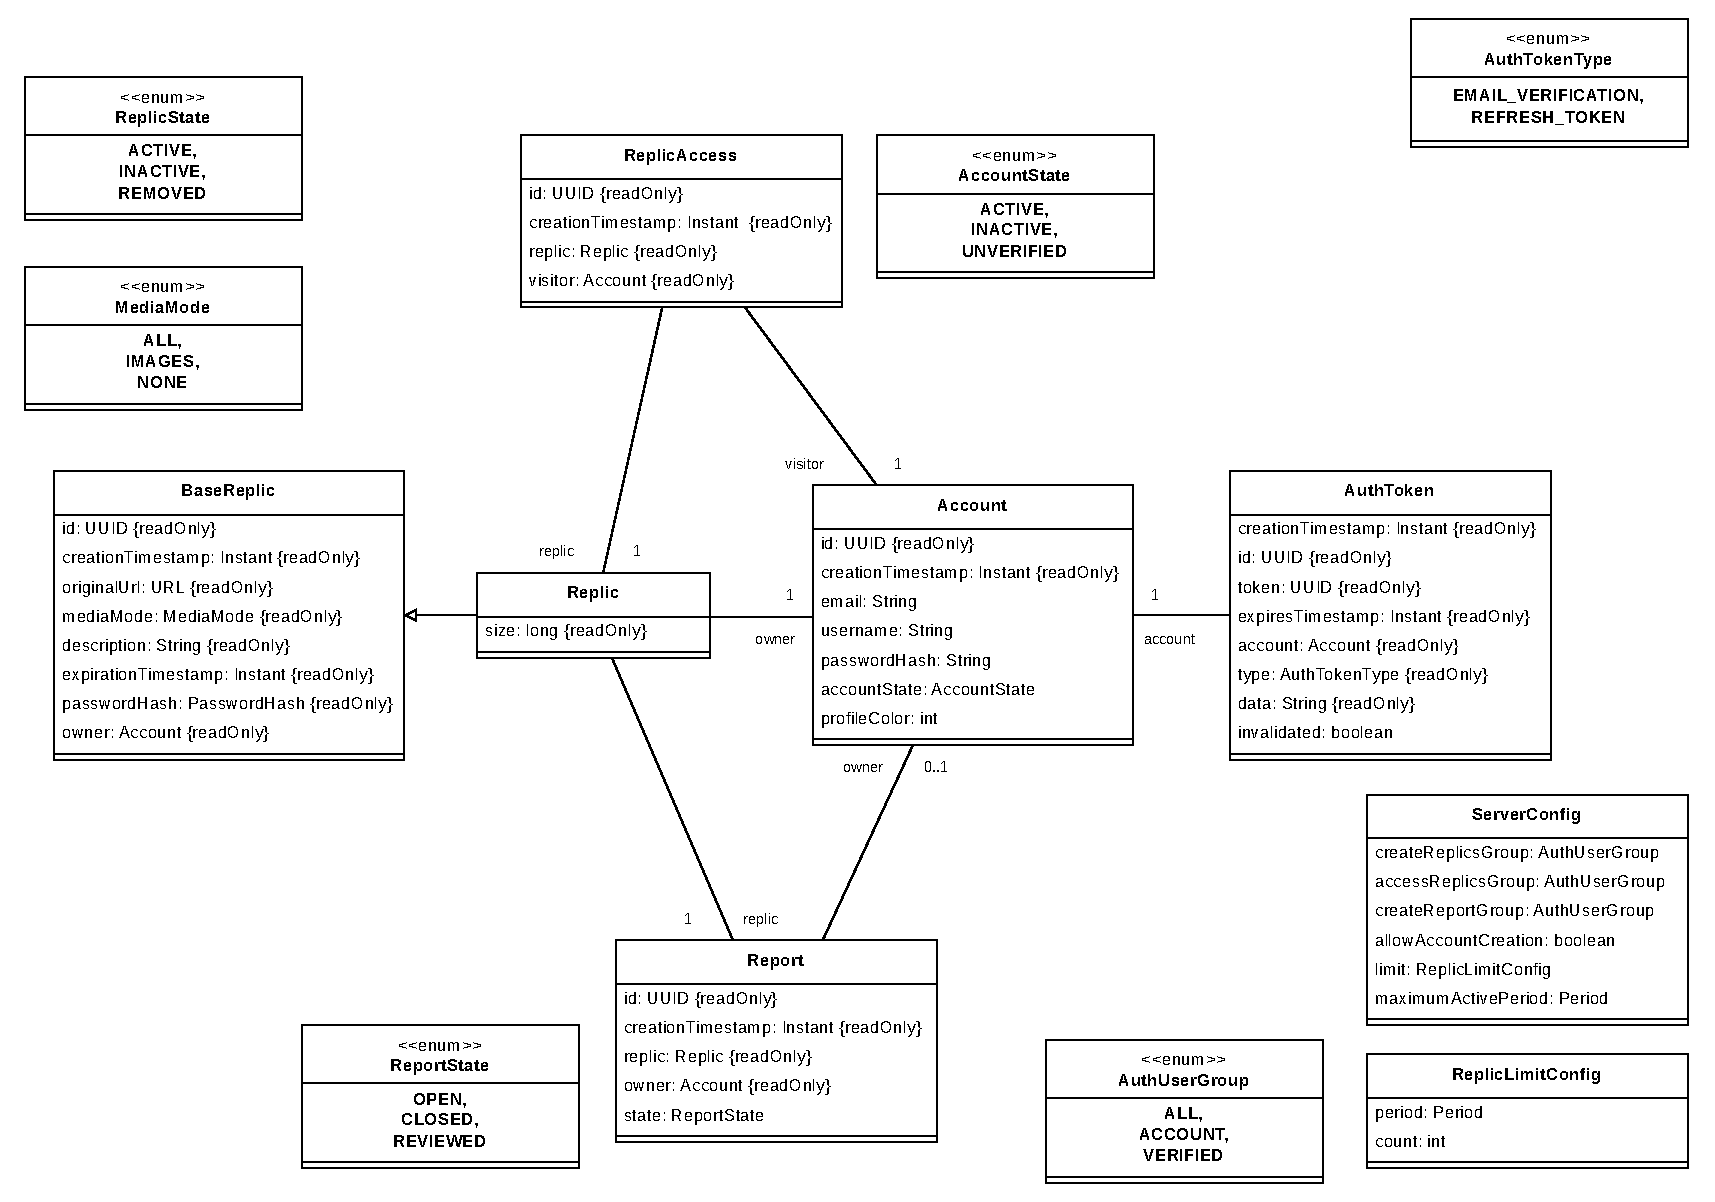
\includegraphics[width=\linewidth]{domain-models}}

    \caption{Interface for \textit{Domain-Models}}
    \label{fig:domain-models}
\end{figure}

\paragraph{Domain-Services} \label{par:domain-services}
The domain services encapsulate the general logic of the app. \newline
The methods of the services are held simple to keep the spirit of the domain.
To prevent returning complex result types, errors are raised by throwing checked exceptions.
Every specific type of failure has a custom exception type that is explicitly declared on the method to allow targeted handling.
Figure~\ref{fig:domain-services} shows the services and their methods.

\begin{figure}
    \centering
    \fbox{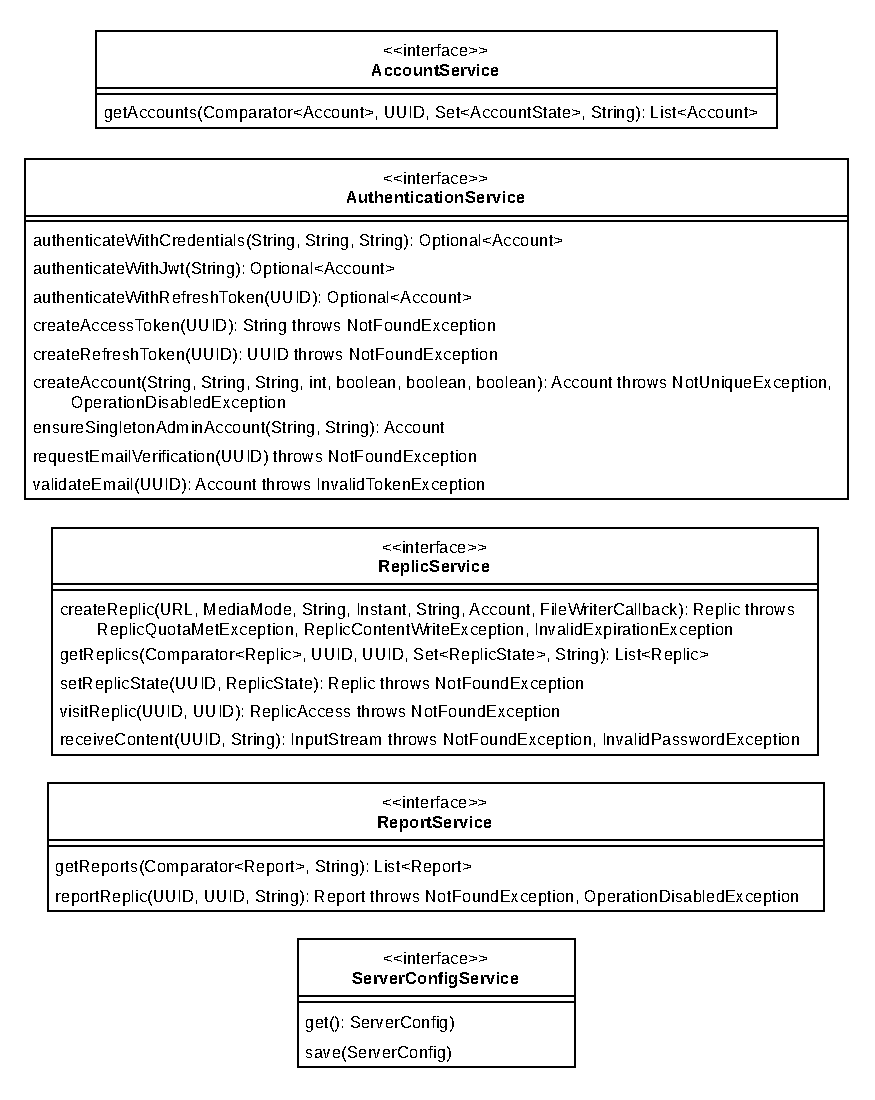
\includegraphics[width=\linewidth]{domain-services}}

    \caption{Interface for \textit{Domain-Services}}
    \label{fig:domain-services}
\end{figure}

\paragraph{Domain-Repositories}\label{par:domain-repositories}
The domain repositories are the way the domain communicates with the database. \newline
Repositories are meant to be a simple interface to queries into a specific table of the relational database.
For most models, it is sufficient to provide the simple methods \texttt{getAll}, \texttt{getById} and \texttt{save}.
Filtering logic is made by the corresponding service.
Figure~\ref{fig:domain-repositories} shows the repository-structure.

\begin{figure}
    \centering
    \fbox{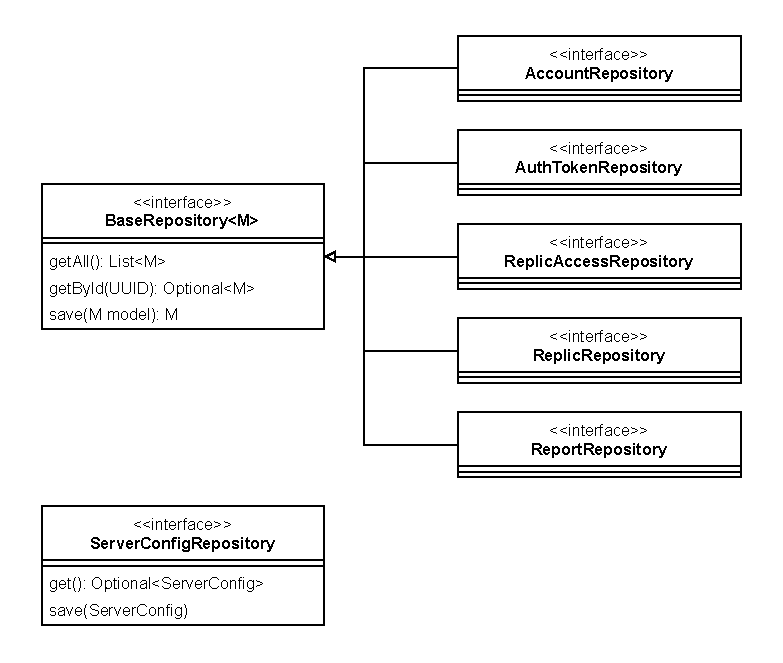
\includegraphics[width=\linewidth]{domain-repositories}}

    \caption{Interface for \textit{Domain-Repositories}}
    \label{fig:domain-repositories}
\end{figure}

\paragraph{Messaging}
The \textbf{Messaging} interface allows to send messages to specified users.
The interface consists of the \textit{EmailSender} as shown in Figure~\ref{fig:domain-messaging}.
Every kind of email corresponds to a method that receives the account to send the email, and required data for the email.

\begin{figure}
    \centering
    \fbox{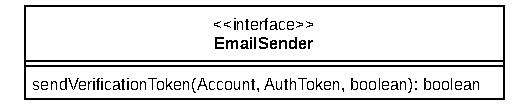
\includegraphics[width=\linewidth]{domain-messaging}}

    \caption{Interface for \textit{Messaging}}
    \label{fig:domain-messaging}
\end{figure}

\paragraph{I/O}\label{par:io}
The \textbf{I/O} interface allows to access and create the files for storing html-content for replics.
The interface consists of the \textit{ReplicFileAccessor} as shown in Figure~\ref{fig:domain-io}.
Simple methods for creating and reading files are there.

\begin{figure}
    \centering
    \fbox{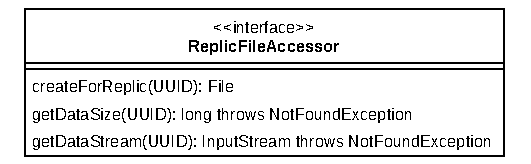
\includegraphics[width=\linewidth]{domain-io}}

    \caption{Interface for \textit{I/O}}
    \label{fig:domain-io}
\end{figure}

\subsubsection{Request-Execution}
The \textbf{Request-Execution} interface is provided by the classes implementing the interfaces (marked with \textit{*Impl}), as shown in Figure~\ref{fig:inter-executors-d}.
The \texttt{AbstractExecutor} class acts as a super class for the executor-implementations by providing access to the \textit{Domain-Services} interface (see~\ref{par:domain-services}).
The executors use the services to access the data.

\begin{figure}
    \centering
    \fbox{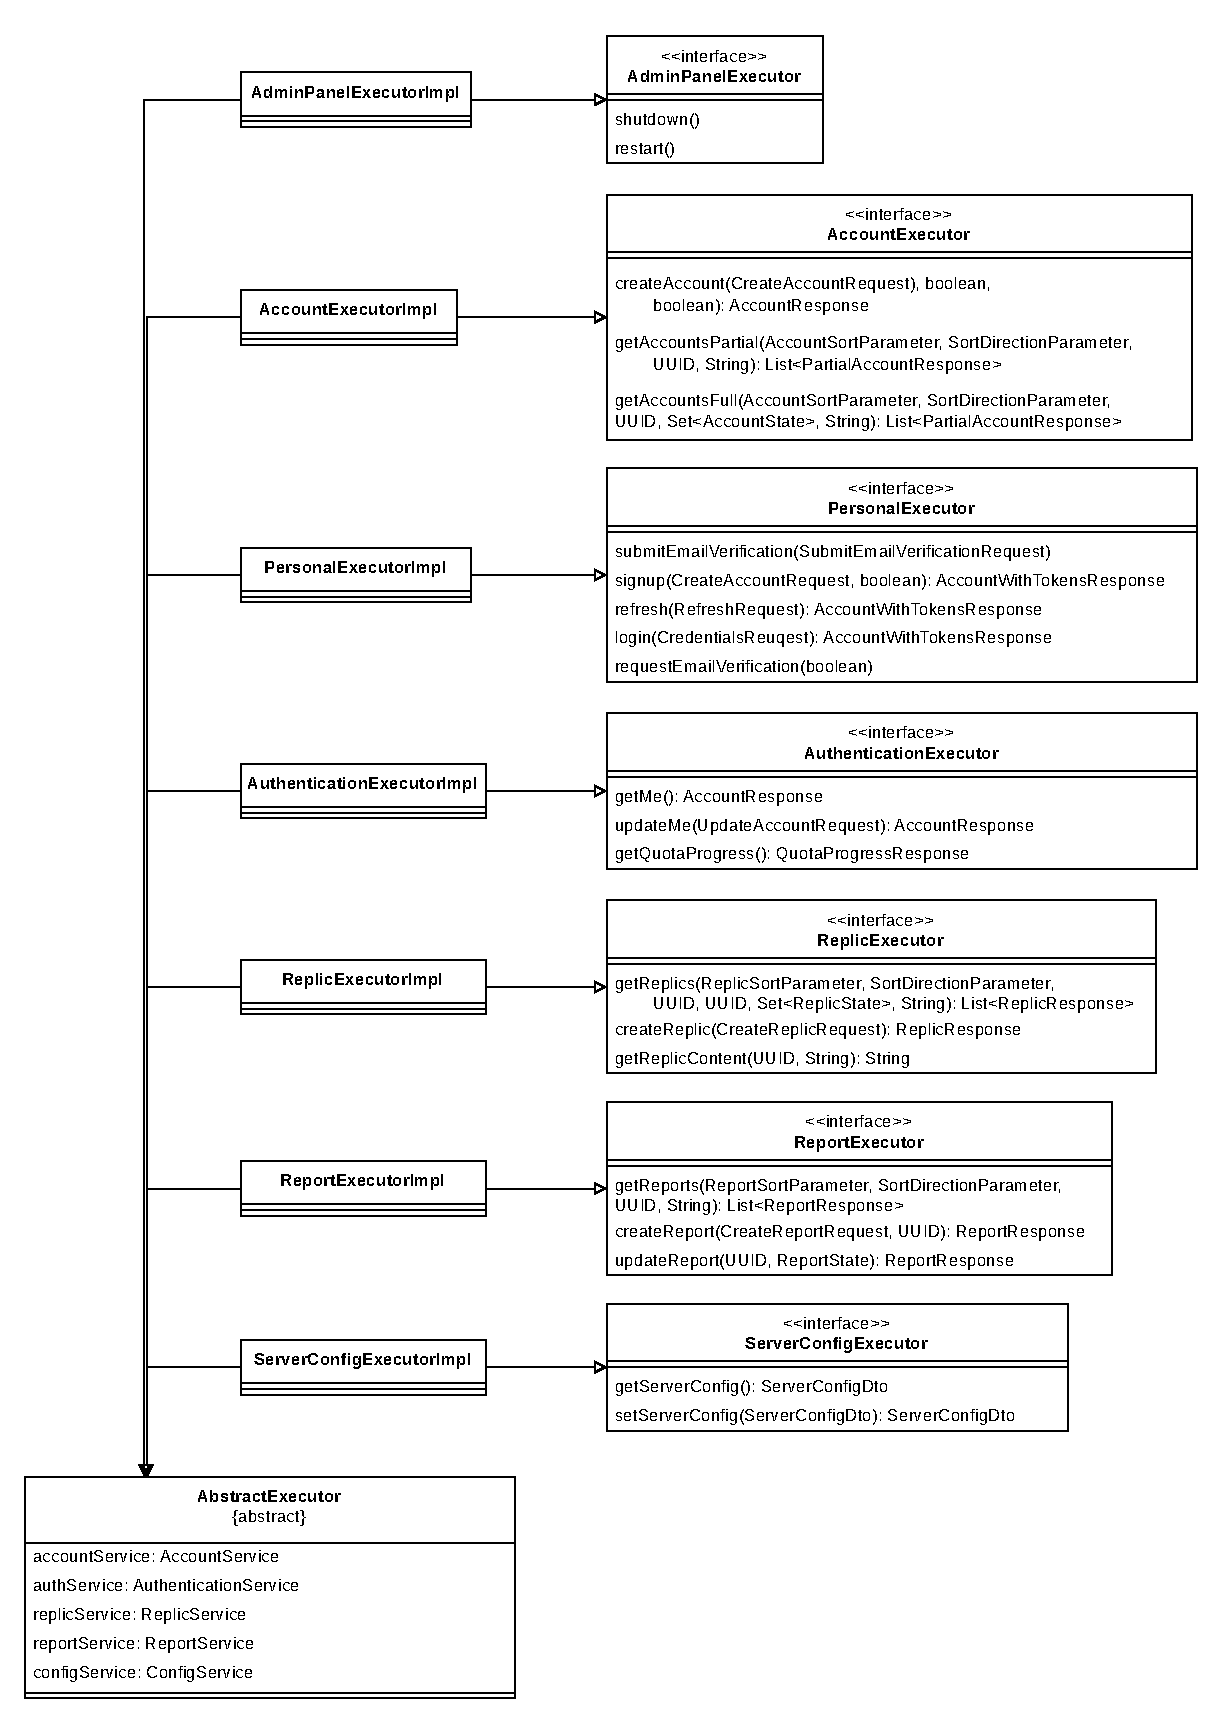
\includegraphics[width=\linewidth]{inter-executors-p}}

    \caption{Provision of \textit{Request-Execution}}
    \label{fig:inter-executors-d}
\end{figure}

\subsubsection{Authorization}
The \textbf{Authorization} interface is provided by the \texttt{RoleGroupBasedAuthorizer}class as shown in~\ref{fig:inter-authorizer-p}.
The class holds a reference to the server-config service (see~\ref{par:domain-services}). \newline
As the name suggests, the implementation is based on roles (for \texttt{canChangeServerConfig} and \texttt{canReviewReports}), and based on admin-checks for the rest.

\begin{figure}
    \centering
    \fbox{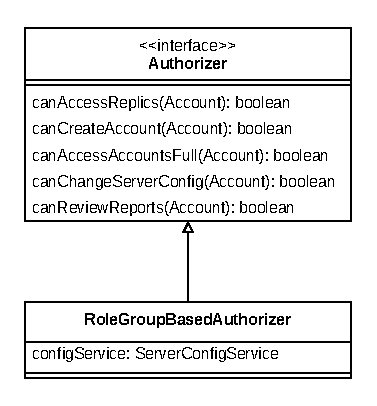
\includegraphics{inter-authorizer-p}}

    \caption{Provision of the \textit{Authorizer}}
    \label{fig:inter-authorizer-p}
\end{figure}

\subsubsection{Domain-Repositories}
The \textbf{Domain-Repositories} interface is provided as shown in Figure~\ref{fig:domain-repositories-p}.
We use the \textit{Adapter pattern} \footnote{https://en.wikipedia.org/wiki/Adapter\_pattern} to delegate the calls. \newline
The adaptee is an instance of a \texttt{CrudRepository<E, UUID>} where \texttt{E} is the appropriate entity-class, e.g. \texttt{ReplicEntity}, that is used in JPA to model a record in a database.
To abstrahize the containing of the adaptee, each implementation class extends the \texttt{BaseJpaAdapter<E>} class.

\begin{figure}
    \centering
    \fbox{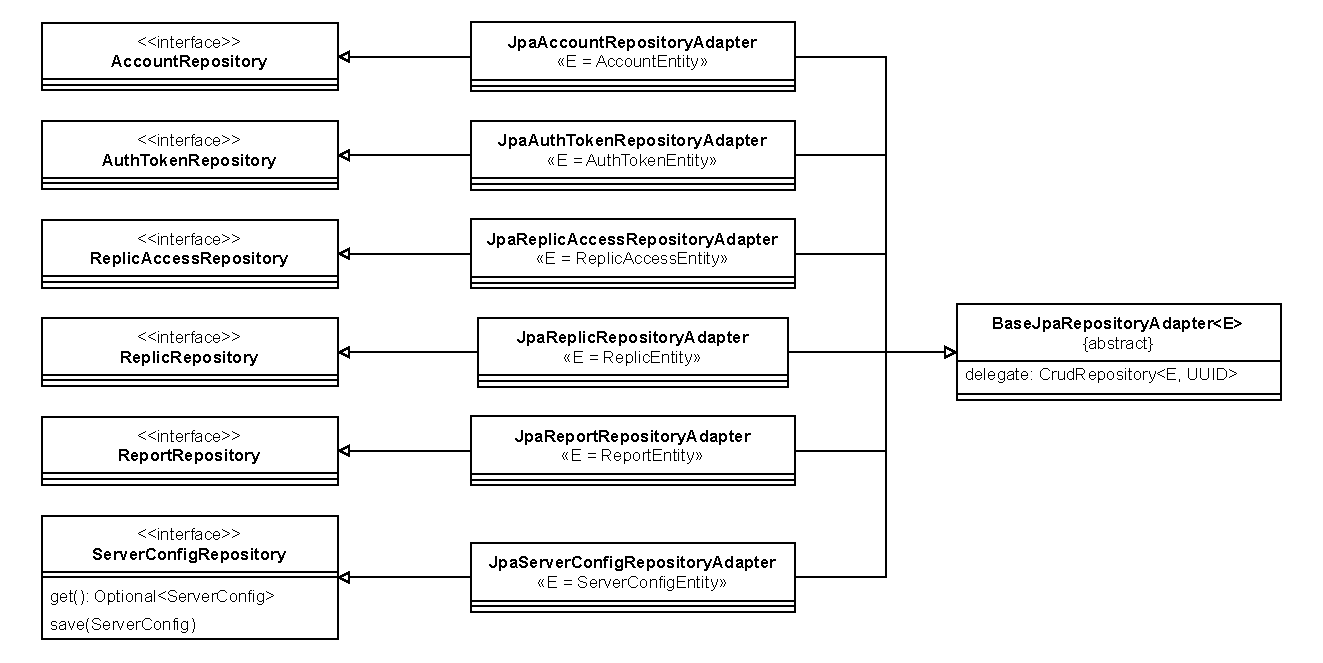
\includegraphics[width=\linewidth]{domain-repositories-p}}

    \caption{Provision of the \textit{Domain-Repositories}}
    \label{fig:domain-repositories-p}
\end{figure}

\subsubsection{Messaging}
The \textbf{Messaging} interface is provided by the \textit{ApacheEmailSender} class as shown in Figure~\ref{fig:domain-messaging-p}.
The class uses the Apache Commons Email library (see~\ref{subsubsec:commons-email}) to send the emails.
As configuration for the email, the parameters \texttt{from}, \texttt{username}, \texttt{password}, \texttt{smtpHost}, \texttt{smtpPort} and \texttt{sslOnConnect} are provided.

\begin{figure}
    \centering
    \fbox{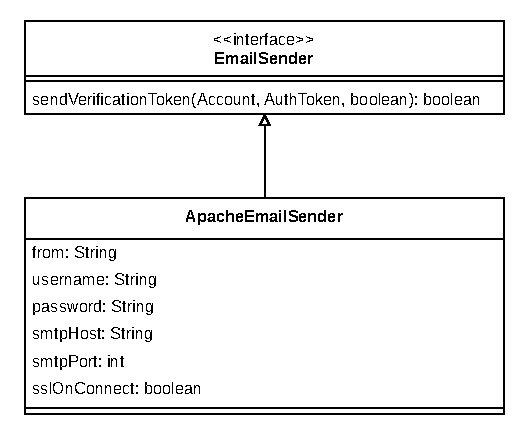
\includegraphics{domain-messaging-p}}

    \caption{Provision of the \textit{Messaging}}
    \label{fig:domain-messaging-p}
\end{figure}

\subsubsection{I/O}
The \textbf{I/O} interface is provided by the \textit{LocalReplicFileAccessor} class as shown in Figure~\ref{fig:domain-io-p}.
The class uses the standard java File-Api \footnote{https://docs.oracle.com/javase/8/docs/api/java/io/File.html} to write and read the files.
The class is provided the \texttt{rootDirectory} string to determine where on the local device the files are saved.

\begin{figure}
    \centering
    \fbox{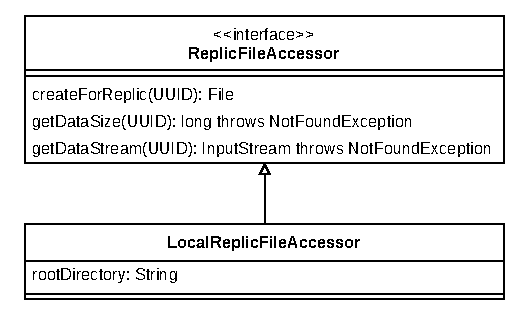
\includegraphics{domain-io-p}}

    \caption{Provision of the \textit{I/O}}
    \label{fig:domain-io-p}
\end{figure}

\subsubsection{Domain-Services}
The \textbf{Domain-Services} interface is provided by several implementation classes as shown in Figure~\ref{fig:domain-services-p}. \newline
The \texttt{AccountServiceImpl} and \texttt{ServerConfigServiceImpl} receive the repositories (see~\ref{par:domain-repositories}) they need to access the database records. \newline
The \texttt{ReplicServiceImpl} and \texttt{ReportServiceImpl} are each provided the config service, and the former one the replic file accessor (see~\ref{par:io}). \newline
The \texttt{AuthenticatioNServiceImpl} has access to the token repository, as well as several other services.
This is allowed as no circular definition occurs, and legitimate as authentication is more abstract than the other operations.
Additionally, it is provided the configuration values \texttt{accessTokenExpiration}, \texttt{refreshTokenExpiration} and \texttt{accessTokenSecret} which are required for the authentication setups.

\begin{figure}
    \centering
    \fbox{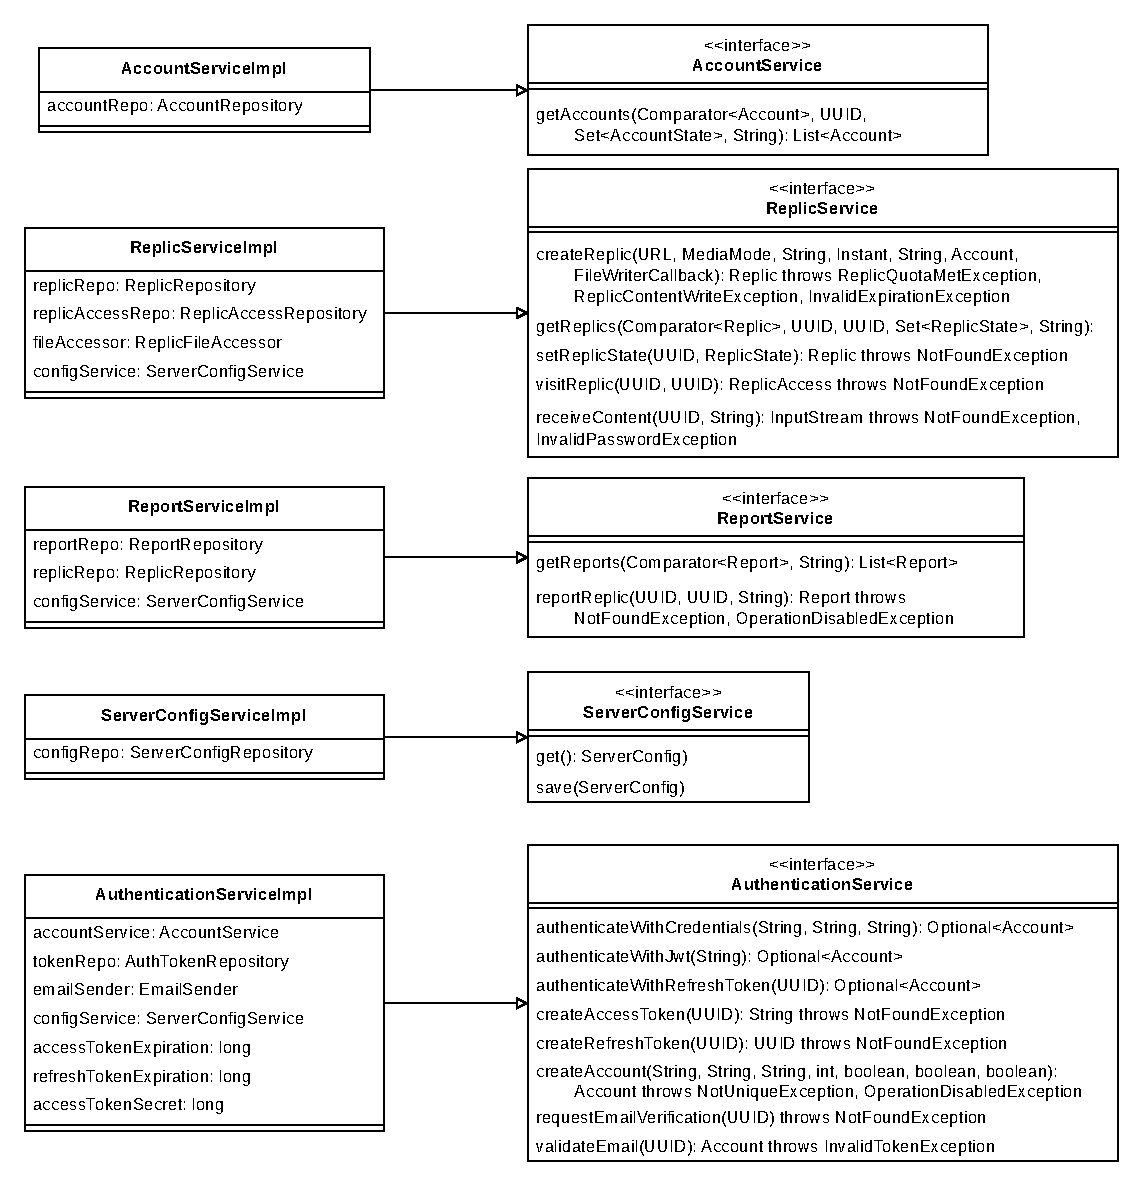
\includegraphics[width=\linewidth]{domain-services-p}}

    \caption{Provision of the \textit{Domain-Services}}
    \label{fig:domain-services-p}
\end{figure}

\subsection{Client fine design}\label{subsec:client-fine-design-common}

\subsubsection{Client internal interfaces}
In the following, we will present the fine design of the internal server interfaces, as described in~\ref{subsec:internal-client-interfaces}.

\paragraph{Network-Interface}\label{par:common-networkinterface}
The \textit{Network-Interface} provides streamlined access to all relevant endpoints and http-methods on the \textit{REST-API}, as shown in Figure~\ref{fig:common-networkinterface}.
Per endpoint and http-method, there is one method whose parameters are the request body, path variables or query paremetr.
The return type of the methods are \texttt{Observable<T>}s from \textit{RxJs} \footnote{https://rxjs.dev/guide/observable} that contain the response body of the request.

\begin{figure}
    \centering
    \fbox{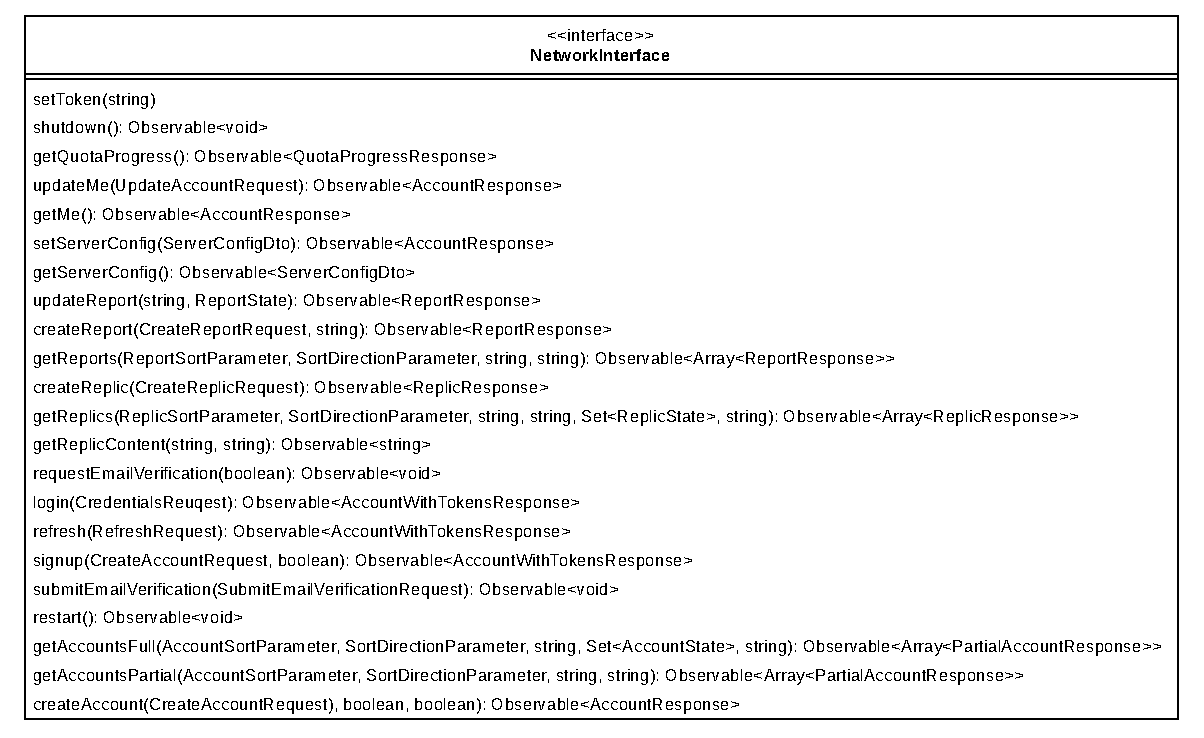
\includegraphics[width=\linewidth]{common-networkinterface}}

    \caption{Interface of \textit{Network-Interface}}
    \label{fig:common-networkinterface}
\end{figure}

\paragraph{Domain-Models}\label{par:common-domain-models}
The \textit{Domain-Models} provides a collection of rich data objects that model the business data of the application, as shown in Figure~\ref{fig:common-domain-models}.
The domain models are the classes that will be used around the app, mostly in the \textit{ViewModel}s. \newline
Due to the different amount of data exposed concerning the authenticated user, and other users, we differentiate between the \textit{PartialAccount} and the normal \textit{Account}.

\begin{figure}
    \centering
    \fbox{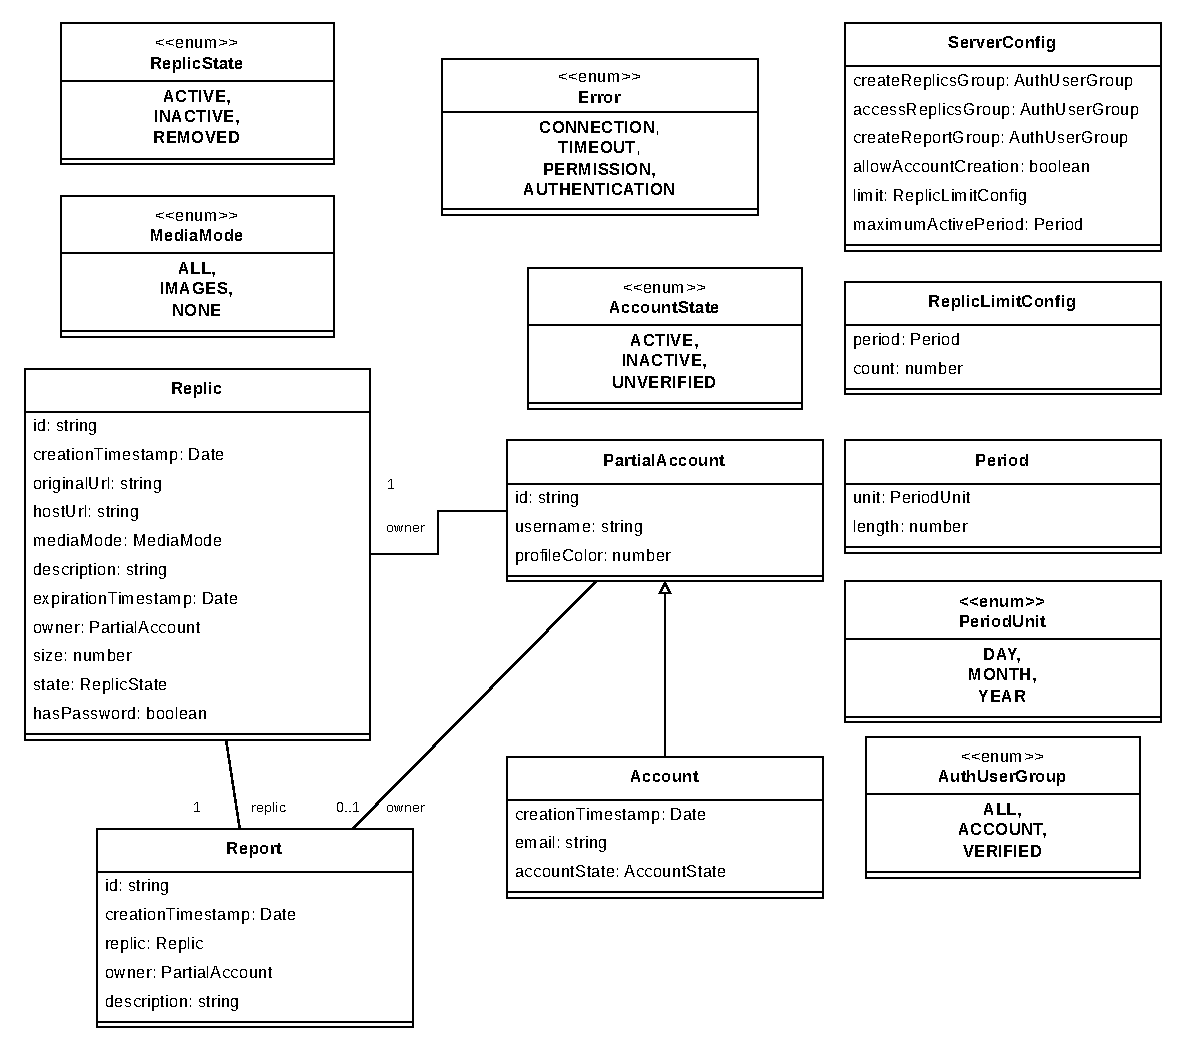
\includegraphics[width=\linewidth]{common-domain-models}}

    \caption{Interface of \textit{Domain-Models} (Client)}
    \label{fig:common-domain-models}
\end{figure}

\paragraph{Authentication-Service}\label{par:common-authentication-service}
The \textit{Authentication-Service} provides methods related to authentication and the authenticated account, as shown in Figure~\ref{fig:common-authentication-service}. \newline
The interface also contains specific errors that are returned from the methods in case the operation fails. \newline
At the core of the \textit{Authentication-Service} is the \texttt{save<T>(NetworkInterface, () => Observable<T>): Observable<T>} method.
It allows the user to perform a method on a specific \texttt{NetworkInterface} without worrying about authentication: if the request fails, and the error my have been caused by a lack of authentication, the token in the network-interface is updated and the request performed again.

\begin{figure}
    \centering
    \fbox{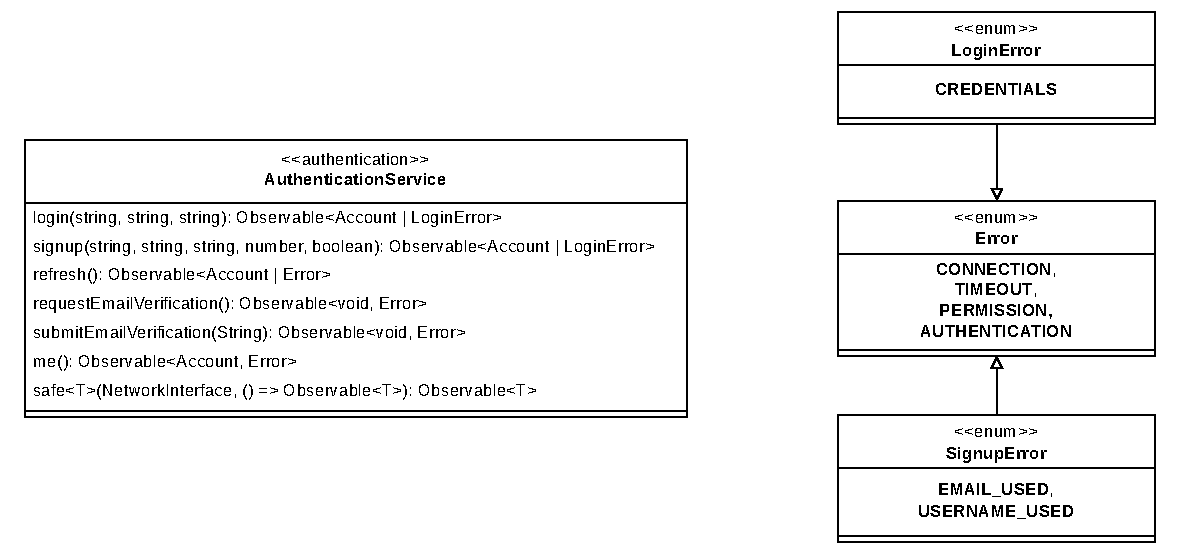
\includegraphics[width=\linewidth]{common-authentication-service}}

    \caption{Interface of \textit{Authentication-Service} (Client)}
    \label{fig:common-authentication-service}
\end{figure}

\paragraph{Data-Services}\label{par:common-data-services}
The \textit{Data-Services} provides all access to the data that is being displayed and updated by the clients.
The interface consists of multiple services as shown in Figure~\ref{fig:common-data-services}. \newline
The interface also provides some specialized error types that make the error-handling easier.

\begin{figure}
    \centering
    \fbox{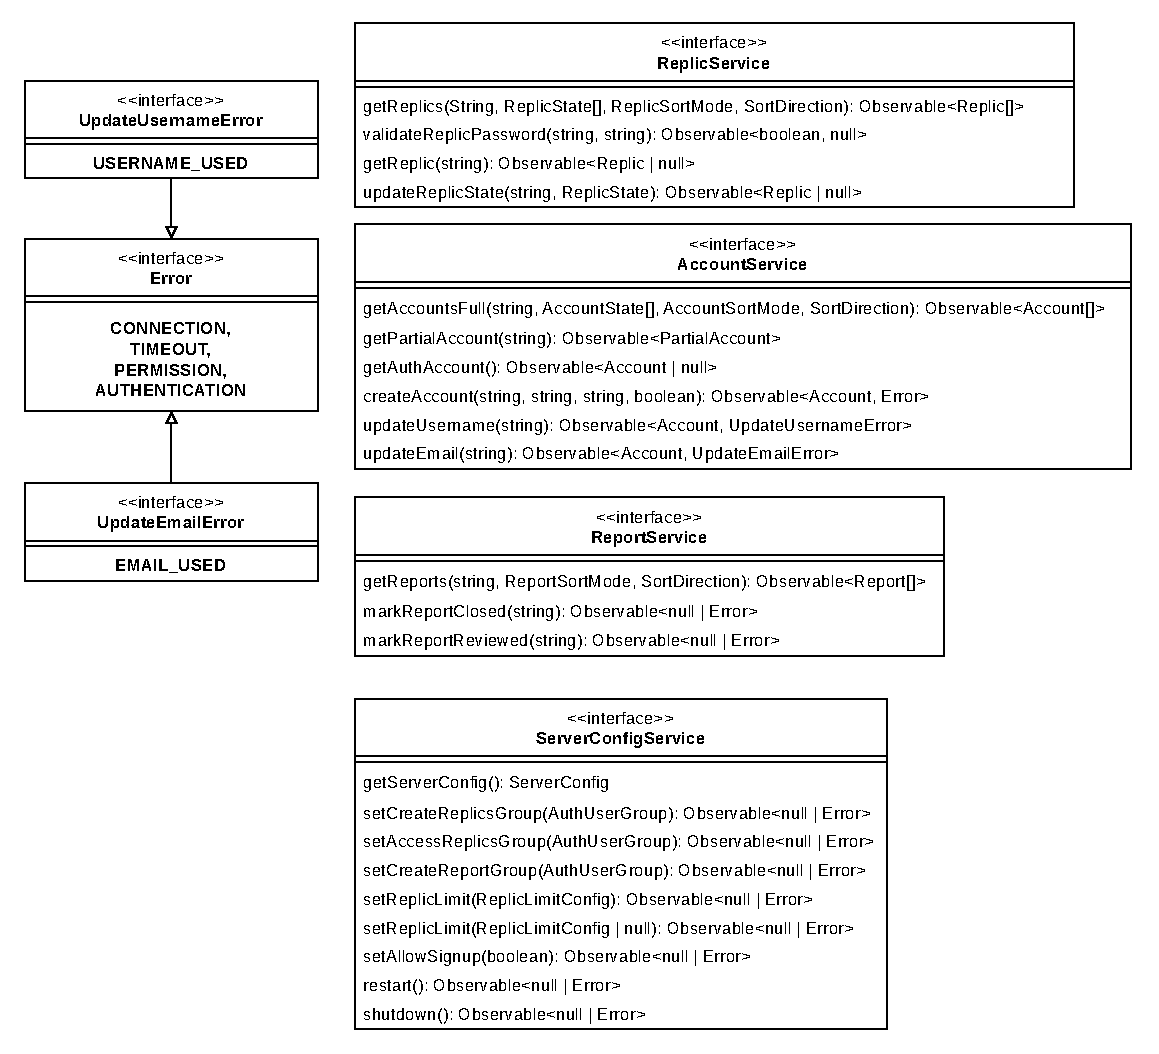
\includegraphics[width=\linewidth]{common-data-services}}

    \caption{Interface of \textit{Data-Services} (Client)}
    \label{fig:common-data-services}
\end{figure}

\paragraph{Common-Facade}
The \textit{Common-Facade} interface bundles the already introduced interfaces \textit{Data-Services} (\ref{par:common-data-services}), \textit{Authentication-Service} (\ref{par:common-authentication-service}) and \textit{Domain-Models} (\ref{par:common-domain-models}).

\paragraph{Config-Service}\label{par:active-config-service}
The \textit{Config-Service} exposes functionality to locally save the settings of the active client.
As shown in Figure~\ref{fig:active-config-service}, the only configuration is the URL of the backend server.

\begin{figure}
    \centering
    \fbox{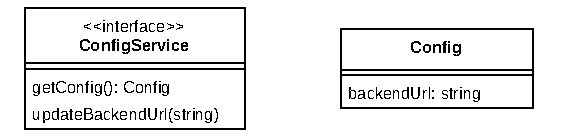
\includegraphics{active-config-service}}

    \caption{Interface of \textit{Config-Service} (Active Client)}
    \label{fig:active-config-service}
\end{figure}

\paragraph{Scrape-Service}\label{par:active-scrape-service}
The \textit{Scrape-Service} handles creating the singular HTML-file that is sent to the server when creating a replic.
Figure~\ref{fig:active-scrape-service} shows the slim interface, where the only method \texttt{createForCurrentTab} creates this HTML-file.

\begin{figure}
    \centering
    \fbox{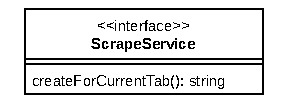
\includegraphics{active-scrape-service}}

    \caption{Interface of \textit{Scrape-Service} (Active Client)}
    \label{fig:active-scrape-service}
\end{figure}

\paragraph{ViewModel}\label{par:viewmodel}
The \textit{ViewModel} interface of both the active and passive client expose \texttt{Signal}s, \texttt{FormControl}s and methods, i.e.\ event-handlers, as shown in Figure~\ref{fig:passive-viewmodel} and Figure~\ref{fig:active-viewmodel}.
These are consumed by the \textit{AngularJS} templates.
For both clients, the \texttt{MainLayoutViewModel} is the \textit{ViewModel} for the layout containing nav-bar and footer, ich which the other views are embedded.
For this reason, despite being displayed in a class-diagram and being marked with \«interface\», they should be seen as a loose collection of fields and methods available to a specific angular-template.

\begin{figure}
    \centering
    \fbox{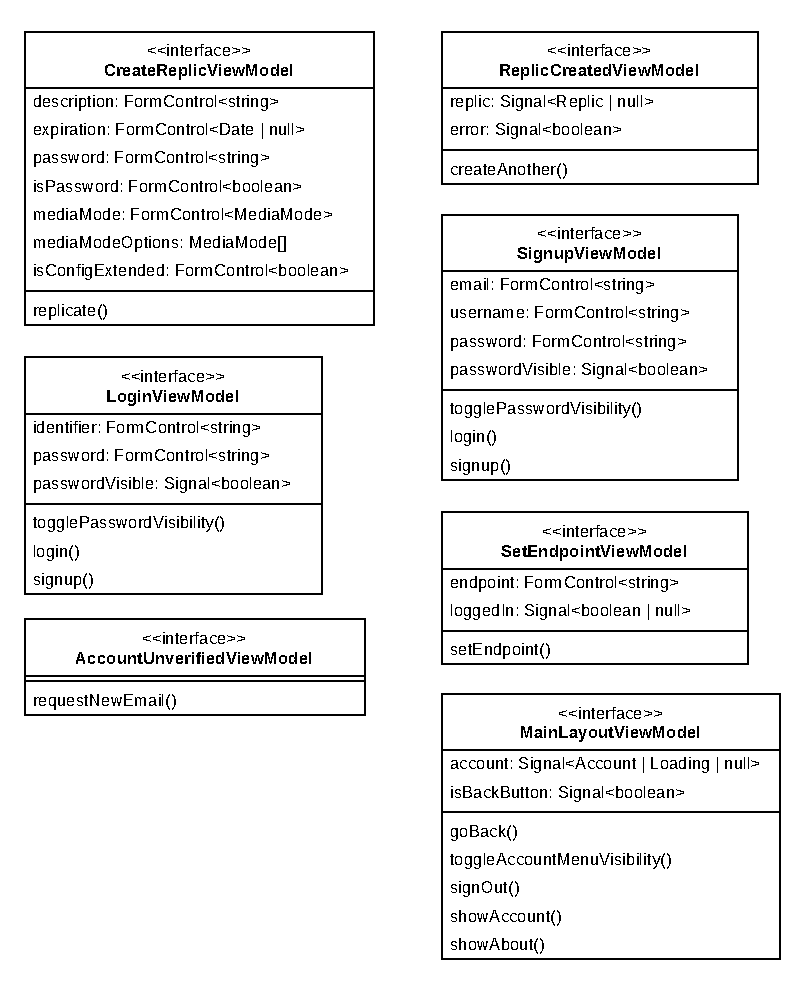
\includegraphics[width=\linewidth]{active-viewmodel}}

    \caption{Interface of \textit{ViewModel} (Active Client)}
    \label{fig:active-viewmodel}
\end{figure}

\begin{figure}
    \centering
    \fbox{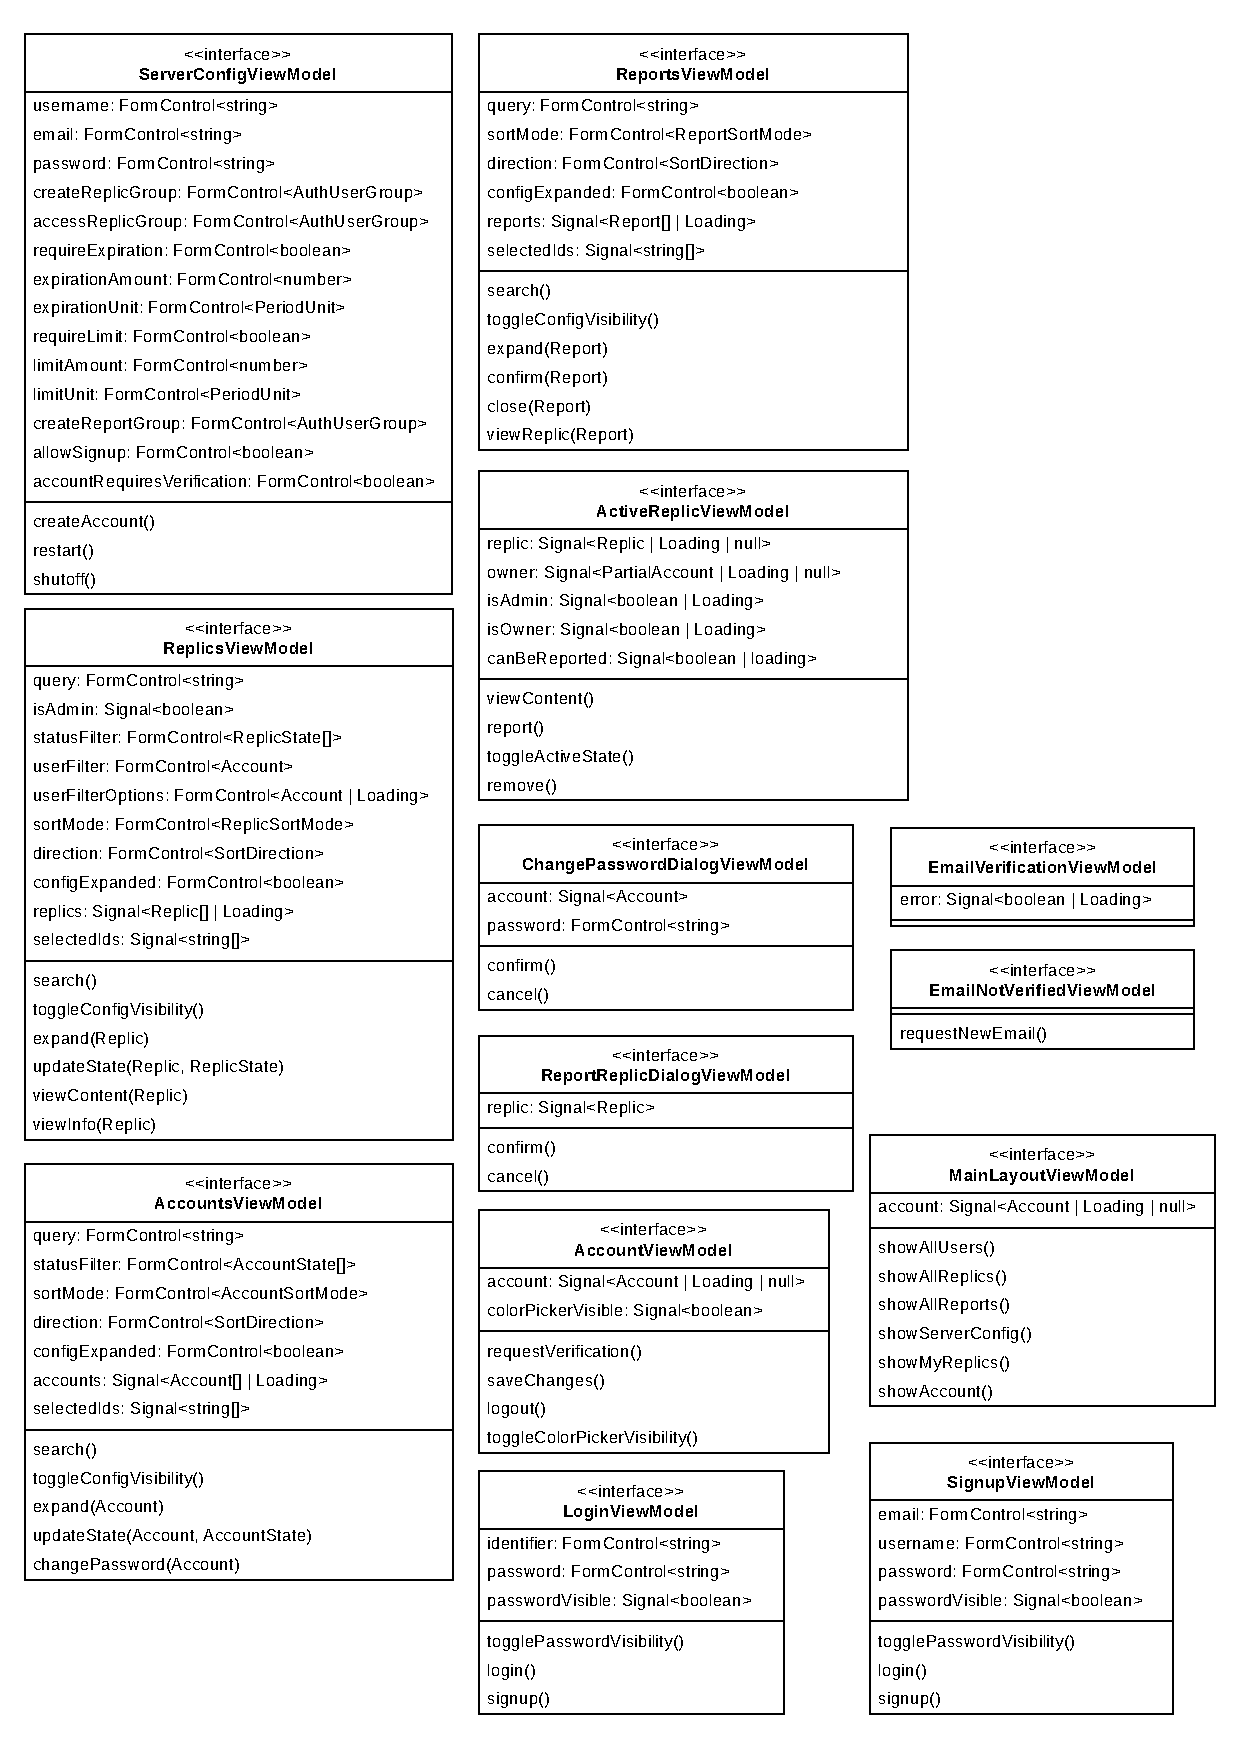
\includegraphics[width=\linewidth]{passive-viewmodel}}

    \caption{Interface of \textit{ViewModel} (Passive Client)}
    \label{fig:passive-viewmodel}
\end{figure}

\subsubsection{Network-Interface}
The \textit{Network-Interface} is provided by the \texttt{AngularHttpNetworkInterface} class, as shown in Figure~\ref{fig:common-networkinterface-p}.
It is backed by an \texttt{HttpClient} \footnote{https://angular.dev/guide/http} from \textit{AngularJs} that is used to perform the http-requests.
The methods delegate calls to the respective endpoint and add necessary headers.

\begin{figure}
    \centering
    \fbox{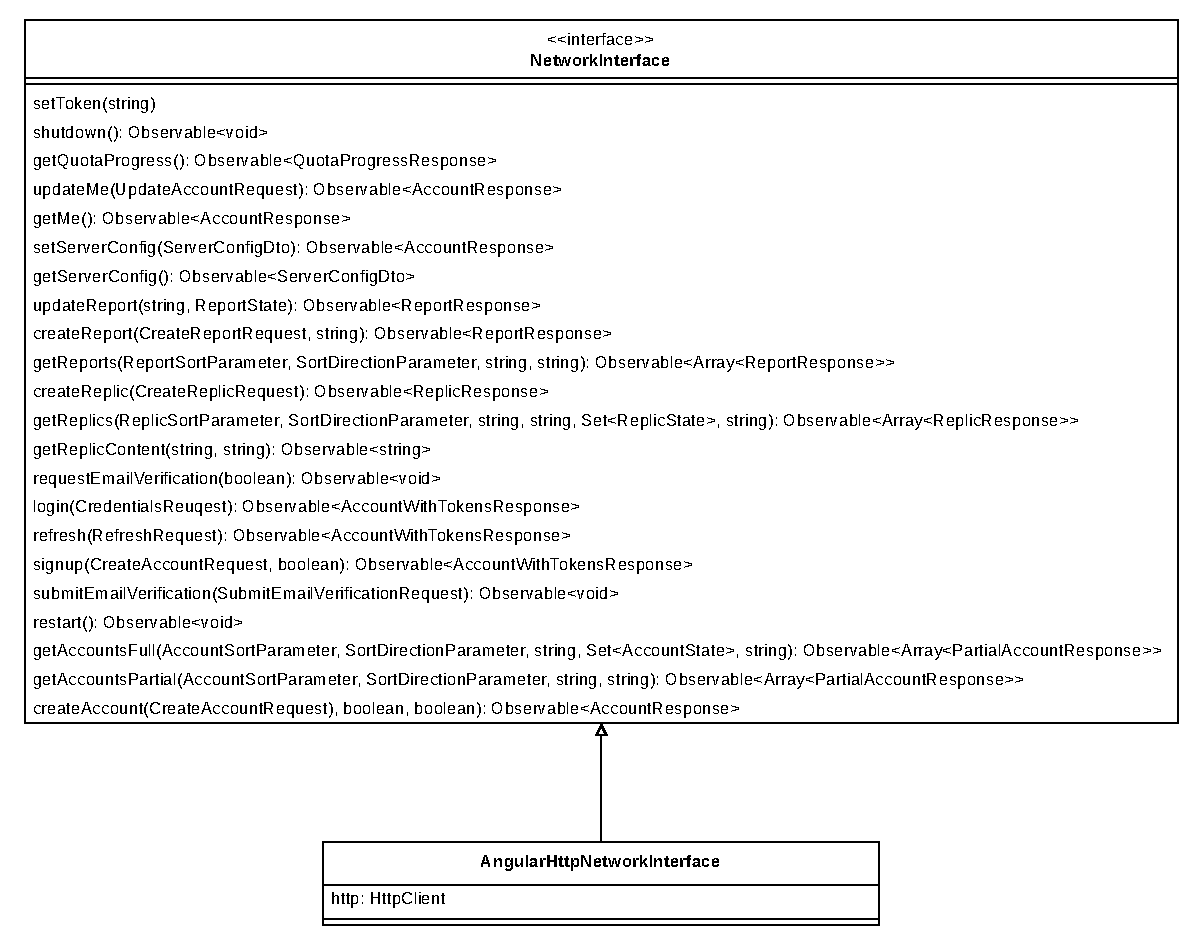
\includegraphics[width=\linewidth]{common-networkinterface-p}}
    \caption{Provision of \textit{Network-Interface} (Client)}
    \label{fig:common-networkinterface-p}
\end{figure}

\subsubsection{Authentication-Service}
The \textit{Authentication-Service} interface is provided by the \texttt{NetworkAuthenticationService}, which is backed by the network-interface as shown in Figure~\ref{fig:common-authentication-service-p}.
The class delegates calls to the network-interface and maps the \textit{HttpErrorResponse}s to \textit{Error}s.

\begin{figure}
    \centering
    \fbox{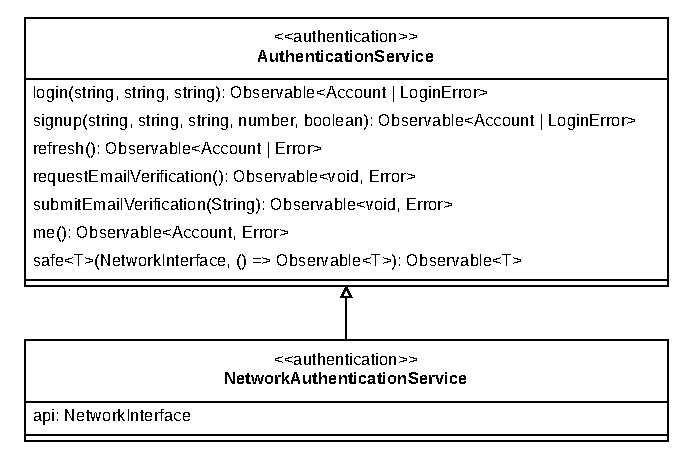
\includegraphics{common-authentication-service-p}}
    \caption{Provision of \textit{Authentication-Service} (Client)}
    \label{fig:common-authentication-service-p}
\end{figure}

\subsubsection{Data-Services}
The \textit{Data-Services} interface is provided by multiple classes as shown in Figure~\ref{fig:common-data-services-p} that implement the interfaces as presented in~\ref{fig:common-data-services}. \newline
The \texttt{BaseDataService} acts as a base that ensures every service has access to the authentication service and network interface, by which the implementations are backed.
The implementations will call the required endpoints and use the \texttt{save} method of the authentication service to ensure proper authentication.
Errors and response bodies will be mapped to the domain-models.

\begin{figure}
    \centering
    \fbox{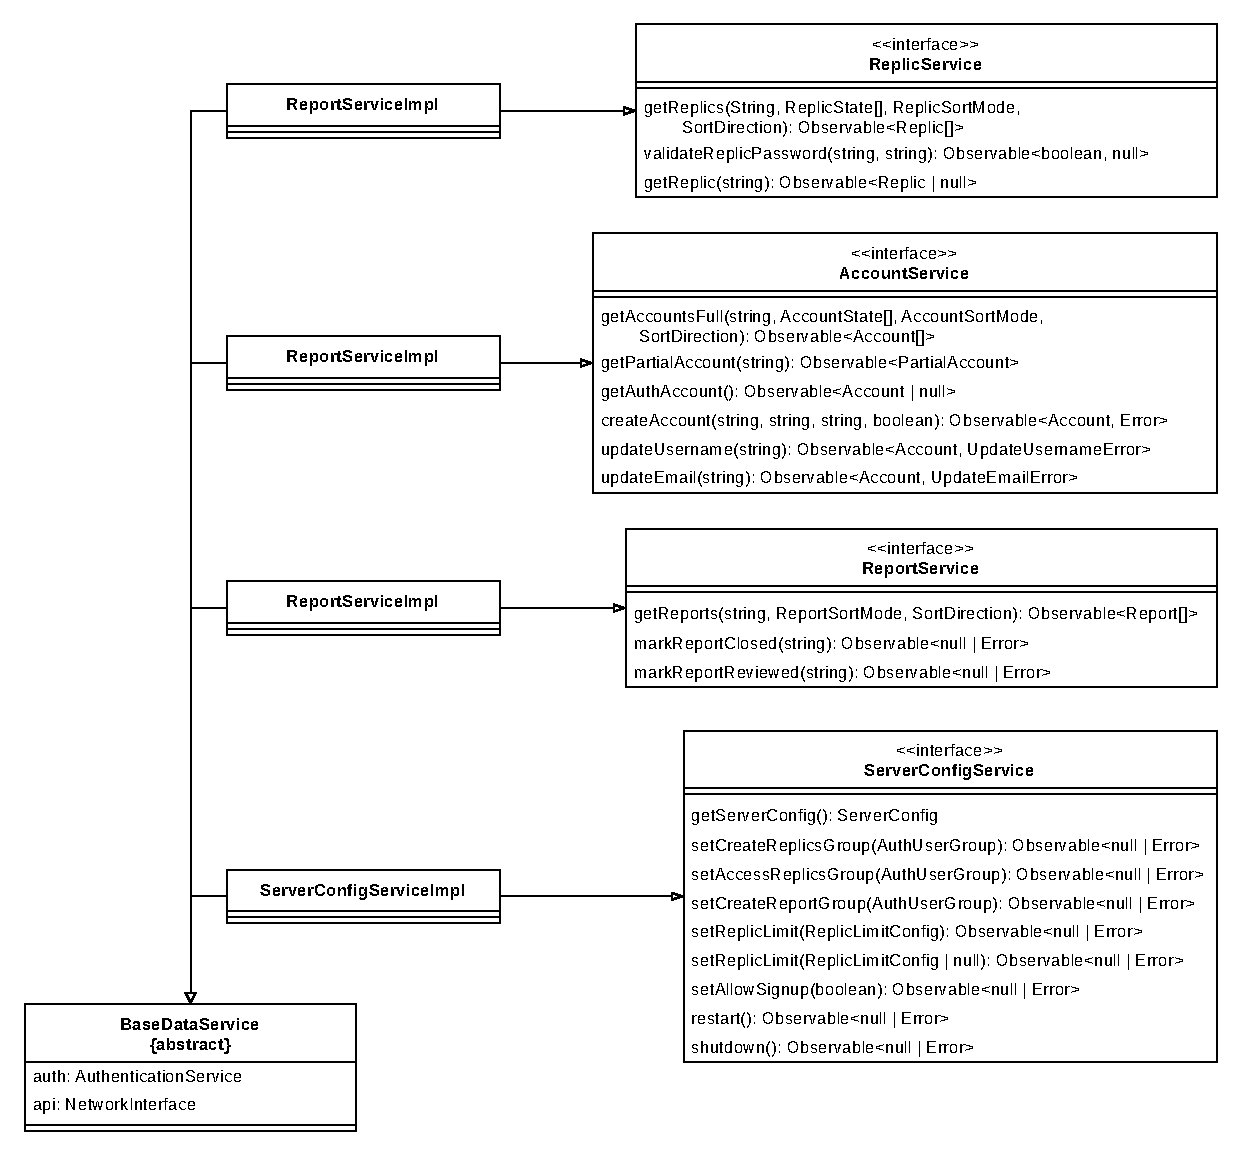
\includegraphics[width=\linewidth]{common-data-services-p}}
    \caption{Provision of \textit{Data-Service} (Client)}
    \label{fig:common-data-services-p}
\end{figure}

\subsubsection{Config-Service}
How the \textit{Config-Service} is provided depends on the current browser the extension is running in.
For chrome, the interface is provided by the \texttt{ChromeStorageConfigService} that is backed by the \texttt{chrome.storage} api \footnote{https://developer.chrome.com/docs/extensions/reference/api/storage}.
For firefox, the interface is provided by the \texttt{FirefoxStorageConfigService} that is backed by the \texttt{storage} api \footnote{https://developer.mozilla.org/en-US/docs/Mozilla/Add-ons/WebExtensions/API/storage}. \newline
Both implementations use the browser-specific storage api to save key-value pairs.
The structure is shown in Figure~\ref{fig:active-config-service-p}.

\begin{figure}
    \centering
    \fbox{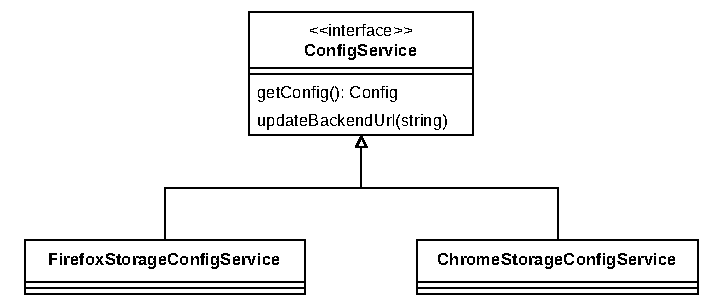
\includegraphics{active-config-service-p}}
    \caption{Provision of \textit{Config-Service} (Client)}
    \label{fig:active-config-service-p}
\end{figure}

\subsubsection{Scrape-Service}
The \textit{Scrape-Service} is provided by the \texttt{TabsScrapeService} whose implementation is backed by the \textit{tabs} api \footnote{https://developer.mozilla.org/en-US/docs/Mozilla/Add-ons/WebExtensions/API/tabs}.
The service pulls the html-content of the current tab and performs some pre-processing, like embedding the referenced scripts and stylesheets.
Figure~\ref{fig:active-scrape-service-p} shows the structure.

\begin{figure}
    \centering
    \fbox{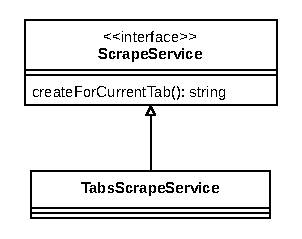
\includegraphics{active-scrape-service-p}}
    \caption{Provision of \textit{Scrape-Service} (Client)}
    \label{fig:active-scrape-service-p}
\end{figure}